The texts in this collection were recorded among the Modole people of Halmahera Island at the beginning of the twentieth century in the context of the mission of the Utrechtse Zendingsvereeniging (UZV). They were published by the missionary G.J. Ellen under the title \textit{Verhalen en fabelen in het Modòle met vertalingen} (`Tales and fables in Modole with translations') in the journal \textit{Bijdragen tot de Taal-, Land- en Volkenkunde van Nederlandsch-Indië} in 1916. Together with a Modole wordlist, published in the same journal, and another wordlist\footnote{One of the Holle lists, published in \citet{stokhof1980, stokhof1980a}.} they remain to this day the only printed publications in or about the Modole language. The aim of this book is to make the texts accessible to a larger linguistic audience. 

The context in which the texts were collected is not documented. Neither the name(s) of the narrator(s) nor the exact time and place of recording is known. To amend this lack of documentation I provide background information about the Modole and their language (Chapter \ref{chap:Modole}), about G.J. Ellen and his mission (Chapter \ref{chap:Ellen}), and about the texts themselves (Chapter \ref{chap:stories}). 
I also include an extensive sketch grammar (Chapter \ref{chapter:sketch}) -- the first published grammatical description of Modole. 
Next are the 10 texts (Part \ref{part:texts}); each with a short introduction and summary, Ellen's original Dutch translation, my English translation, and the interlinearlized Modole text. Notes on the texts are provided in footnotes.
Throughout this book, I refer to the Malay varieties spoken in Indonesia as \textit{Indonesian}, even though the texts precede the Indonesian nation state. 

\chapter{The Modole, their land and their language}
\label{chap:Modole}

In this chapter, I provide information about the history of the Modole people (\sectref{subsec:people}), their traditional religious customs and folk tale traditions (\sectref{subsec:folk_religion}), their geographical surroundings (\sectref{subsec:land}) and their language (\sectref{subsec:land}).
Much of this information comes from colonial sources, often written in the condescending and patronizing tone common to these sources. 

\section{History of the Modole people}
\label{subsec:people}

The Modole are one of the ethnic groups (Indonesian \textit{suku}) of the northern peninsula of Halmahera island. Halmahera is part of the North Moluccas in modern-day eastern Indonesia. The Modole have occupied an area along the upper Kao river in the modern district Kao Barat since at least the 17th century. They were formerly subjects of the Sultan of Ternate, an island to the west of Halmahera that gained power and wealth through the spice trade. The North Moluccas are the native home of the clove tree (\textit{Syzygium aromaticum}) and traders from Java, India, China, Arabia and Europe visited the islands in medival and early modern times to buy the precious commodity.  

Since they lived far in the interior of Halmahera, the Modole remained outside the focus of European colonizers longer than their neighbors. 
They are first mentioned in an European source in a report by the retiring Dutch Governor of Ternate, Jacob Lobs, dating to 1686 (published in \cite{dam1931}). Lobs mentions a place-name called \textit{Mondole} two hours away from Pagu. The inhabitants are described as ``wilt, schuw en vreesagtig'' (`wild, shy and apprehensive', \cite[113]{dam1931}). There were 30 able-bodied men among them.

After Lobs' report, the Modole are not mentioned in European sources until the 19th century.
For the end of the 19th century, \citet[62, 66]{declercq1890} states that the \textit{sangaji} (a kind of local ruler) of the district Modole (spelled Madolé) is subject to the \textit{sangaji} of Kao Bay, and that the \textit{negorij} (small village) Madolé does not pay regular taxes to the Sultan of Ternate (its formal ruler).

According to \citet{ellen1916}, there were around 2,000 Modole at the beginning of the 20th century.\footnote{Precise numbers of Modole congregation members can be found in \citet[136]{utrechtschezendingvereeniging1915}. I decided against including them here since they only cover Christians and hence a fraction of the total Modole population.}
In 1909, the \textit{Civiele Gezaghebber} (administrator) of the east coast of Halmahera, G.J.J. de Jongh, included several traditions about the origin of the Modole in one of his reports. 
He states that they are related to the Tabaru and ``came from elsewhere with them, likely from Sulawesi, because the Madole are still called `orang bugis' [Buginese]'' \citep[755]{dejongh1909}.\footnote{``met deze van elders kwamen, waarschijnlijk van Celebes, want de Madolé's worden thans nog wel door de anderen `orang boegies' genoemd''}
There were immigrants from Sulawesi in the area around the time, but a connection to the Modole is not mentioned elsewhere. 
De Jongh further reports that the villages Gogala ma lako, Bailengit and Tolabit, which today are inhabited by Modole, were founded by people who originally lived around Lake Lina (see Map in \figref{fig:villages}). Other inhabitants of the Lake Lina area became the modern-day Tobelos, implying that Modole and Tobelo have a shared origin \citep[756]{dejongh1909}. The story is considered implausible by \citet[125-126]{vanfraassen1980} on linguistic grounds. 
According to \citet[756]{dejongh1909}, the Modole from the villages of Toegoeis (Tuguis), Hoekoem (Soahukum), Sengadji (Soasengaji) and Taraut (Torawat) originally lived with the Gamkonora and were attracted by the Sago forests in the Modole region. \citet{leith1999} also corroborates that the population of Torawat were immigrants.

The Modole had an infamous reputation in the early 20th century.
In 1906, UZV missionary G.J. Ellen reported that he had not been able to visit the Modole yet ``since all other tribes are scared of these people''\footnote{``omdat alle anderen stammen bang zijn voor deze menschen''} \citep[166]{ellen1906}.
De Jongh, however, had visited the Modole and Ellen states that ``from his reports, as well as those of the gurus\footnote{helpers from other parts of Indonesia (MZ)} and my own observations it seems that this tribe is not as hostile as thought. It mostly seems to be incitement of the Mohammedans, who want to use this rather large tribe in their hatred of Christianity and the government''\footnote{``Uit zijne mededeelingen, alsmede die der goeroes en mijn eigen bevindingen is mij gebleken dat die stam niet zoo vijandig is als wel werd vermoed. Het schijnt veelal opstokerij van de Mohammedanen te zijn, die dezen tamelijk grooten stam willen gebruiken in hun haat tegen het Christendom en het Gouvernement.''} \citep[166]{ellen1906}.
It must be noted that local Muslims were seen as antagonists by the Dutch missionaries and were therefore accused of all manner of misdeeds (compare \cite[6-7]{ellennda} and the preface of \cite{ellennd}). 
In any case, the Modole did not live up to the stories that Ellen had been told about them. 
He further reports that Modole from the villages of Perseba and Bailengit wished to become Christians and later, gurus were placed there \citep[166]{ellen1906}.\footnote{For more information on the mission among the Modole see Chapter \ref{chap:Ellen}.}  
%add population numbers from 1915_28_8_9

After the Indonesian independence, interest in the Modole did not increase.
\citet{leith1999} outlines the recent history of the Modole and appears to be the only ethnological study concerning them. A short video filmed in the Modole village Soamahukum in 2022 can be found at \url{https://youtu.be/xfkSKQTlDpQ?si=wzV9ST8u8bBEjQob} (accessed 4 October 2025). The map in Figure \ref{fig:villages} shows the location of the original Modole villages today.\footnote{Due to the transmigration program of the Indonesian government, villages of the same name now exist further south in the Malifut area (see \cite{leith1999}).}

\begin{figure}
    \centering
    \includegraphics[width=1\linewidth]{figures/Modole.png}
    \caption{Position of the original Modole villages today (the village of Soasengaji is now called Sangaji Jaya) [created by the author]}
    \label{fig:villages}
\end{figure}

Unfortunately, no detailed accounts about the daily life of the Modole around the time when the texts were collected are available. When the texts in this collection were recorded, many Modole had only recently come into closer contact with the Dutch colonialists and their Christian faith that they were now encouraged to adopt.
Reports by civil colonial administrators focus on population numbers and taxes, while missionaries like Ellen mostly reported on the progress of Christianization and the changes brought about by it.
For example, one of the prerequisites for becoming Christian was to settle permanently in a village and give up foraging. Before, people had often spent extensive periods of time in their inland gardens and created income by collecting dammar gum \citep[159]{ellen1908}. The most comprehensive ethnographic description of a North Halmaheran ethnic group was published by Ellen's missionary colleague \citet{hueting1921,hueting1922} about the Tobelo people. Many aspects of his description pertain to the Modole as well. 



\section{Modole folk tale tradition and traditional religious beliefs}
\label{subsec:folk_religion}

We may call the texts published in Ellen's (\citeyear{ellen1916}) collection `folk stories'. They show similarities to folk stories collected among other North Halmahera groups. For example, the story \textit{O Biara} (Chapter \ref{chapter:text07}) strongly resembles the story \textit{O Radja-Moloko de o ngo Namo-Bilala ma ngadje-ngadje} (`The story of Raja-Moloko and Namo-Bilala') in \posscitet{fortgens1928} Tabaru story collection.\footnote{Notably, there is no version of the `Monkey and Tortoise' story popular throughout Eastern Indonesia, see \citet[411]{vanstaden2000} for a Tidore version and information on the story in general.} 

Before their conversion to Christianity, the Modole adhered to a religion similar to those of other North Halmaheran ethnic groups. There is no comprehensive study of Modole traditional religious beliefs. Some information is found in \citet{leith1999}.\footnote{Note that the paper is concerned with southern Modole villages, while the texts likely were collected in the northern villages.} Elements of these traditional religious beliefs are still preserved today and have been incorporated into local Christianity. The traditional religious beliefs include ancestor worship as well as the belief in a number of spirits and other supernatural beings.
Some of them populate the enchanted country in which the stories in this collection are set; among them the \textit{to'ata} (a kind of evil spirit), the \textit{goda} spirit, \textit{jini} `jinns' and \textit{widadari} `nymphs' (see footnotes in respective texts for more information). 

The interior of Halmahera may appear remote today but historically it was connected to the world through the spice trade and the Modole adopted many foreign cultural practices.
The belief in jinns had been adopted from Muslims at some point in time. Immigrants from Ternate and local converts lived in the coastal settlements of Kao bay. The protagonists of the text \textit{Naga o njawa ja mididi jo puaha} (Chapter \ref{chapter:text08}) are Muslims.
The word \textit{widadari} is of Javanese (and ultimately Sanskrit) origin. Javanese culture was brought to Ternate by traders and spread from there to Halmahera (see \citet{schapper2025}). 
\citet[12-13]{hueting1908a} believed that many of the Tobelo stories originated elsewhere and observed similarities to stories collected on the Sangir islands north of Sulawesi.

The missionaries further noted that some of the folk stories they recorded appear to be a combination of several stories (see for example \cite[454]{vanbaarda1904}). This was still observed in 2000 by \citet[337]{vanstaden2000}. A candidate for such a combined story is \textref{chapter:text01}.

The \textit{Sitz im Leben} of the stories is not documented.
The only information regarding the function and meaning of folk tales for the daily lives of the people of North Halmahera at the beginning of the 20th century is found in the introduction of Hueting's (\citeyear{hueting1908a}) Tobelo story collection:

\begin{quote}
 ``These stories do not play an important role in the lives of the Tobelo. Only few know them and one can spend quite a long time among them without knowing that such stories are known at all. They are not told during public events or feasts but rather in private circles. Usually this happens -- only in a few families -- at night, when they have already gone to bed but cannot fall asleep. [...] Sometimes someone will say: I know a story. Just tell it, others reply. The story teller starts by saying ``Stories''  and every one replies ``téde'', which means ``we are listening''. Then the story follows. Afterwards the story is dissected, or someone else feels inspired to tell one too, and so it continues until everybody has fallen asleep. [...] In fact, the stories do not feel as real to the people as one may think. [...] Also, what one reads about supernatural matters or about the spirit world and the life hereafter hardly corresponds to the common belief about these things, and I have never known anyone to be the least disturbed by what appears in the stories in this respect, or that anything is claimed based on them. They are an amusement, nothing more.'' \citep[13]{hueting1908a} (my translation)
\end{quote}

One interesting feature of the stories is the large number of assertive female protagonists. Most characters and almost all protagonists are women or girls. For more motives found in the stories, see the footnotes to the interlinearized texts. Several common motives of Loloda folk tales, some of which also occur in the Modole stories, are discussed in \citet[322--329]{vanbaarda1904}.


\section{The Modole land}
\label{subsec:land}

The most detailed description of geographic surroundings of the Modole around the time the texts were recorded can be found in \citet{campen1884}. Ellen's (\citeyear{ellennd}) report of one of his trips to the Modole villages provides further information.
According to \citet[277]{campen1884}, the first Modole village is reached from the coast after eight hours' walk.\footnote{Campen calls it Babawat. This name is not recorded elsewhere.}
The interior of Halmahera was dominated by thick rain forest, as it is today.  Most parts of the island are covered by mountain ranges with several active volcanoes, but the Modole land around the Kao river forms a valley with marshy soil. Rivers constitute the main means of transportation. The largest of these is the Kao river (see Figure \ref{fig:Kao_river}).\footnote{Link to the photograph: \url{http://hdl.handle.net/1887.1/item:829037} (accessed 4 October 2025)} Traveling by boat plays a role in almost all of the stories in the collection. 
Sago forests provided the staple food source at the time (compare \textref{chapter:text03} and \textref{chapter:text05}), supplemented by fishing and hunting (compare \textref{chapter:text02}, \textref{chapter:text03}, see \cite[252-274]{hueting1922}).

\begin{figure}
    \centering
    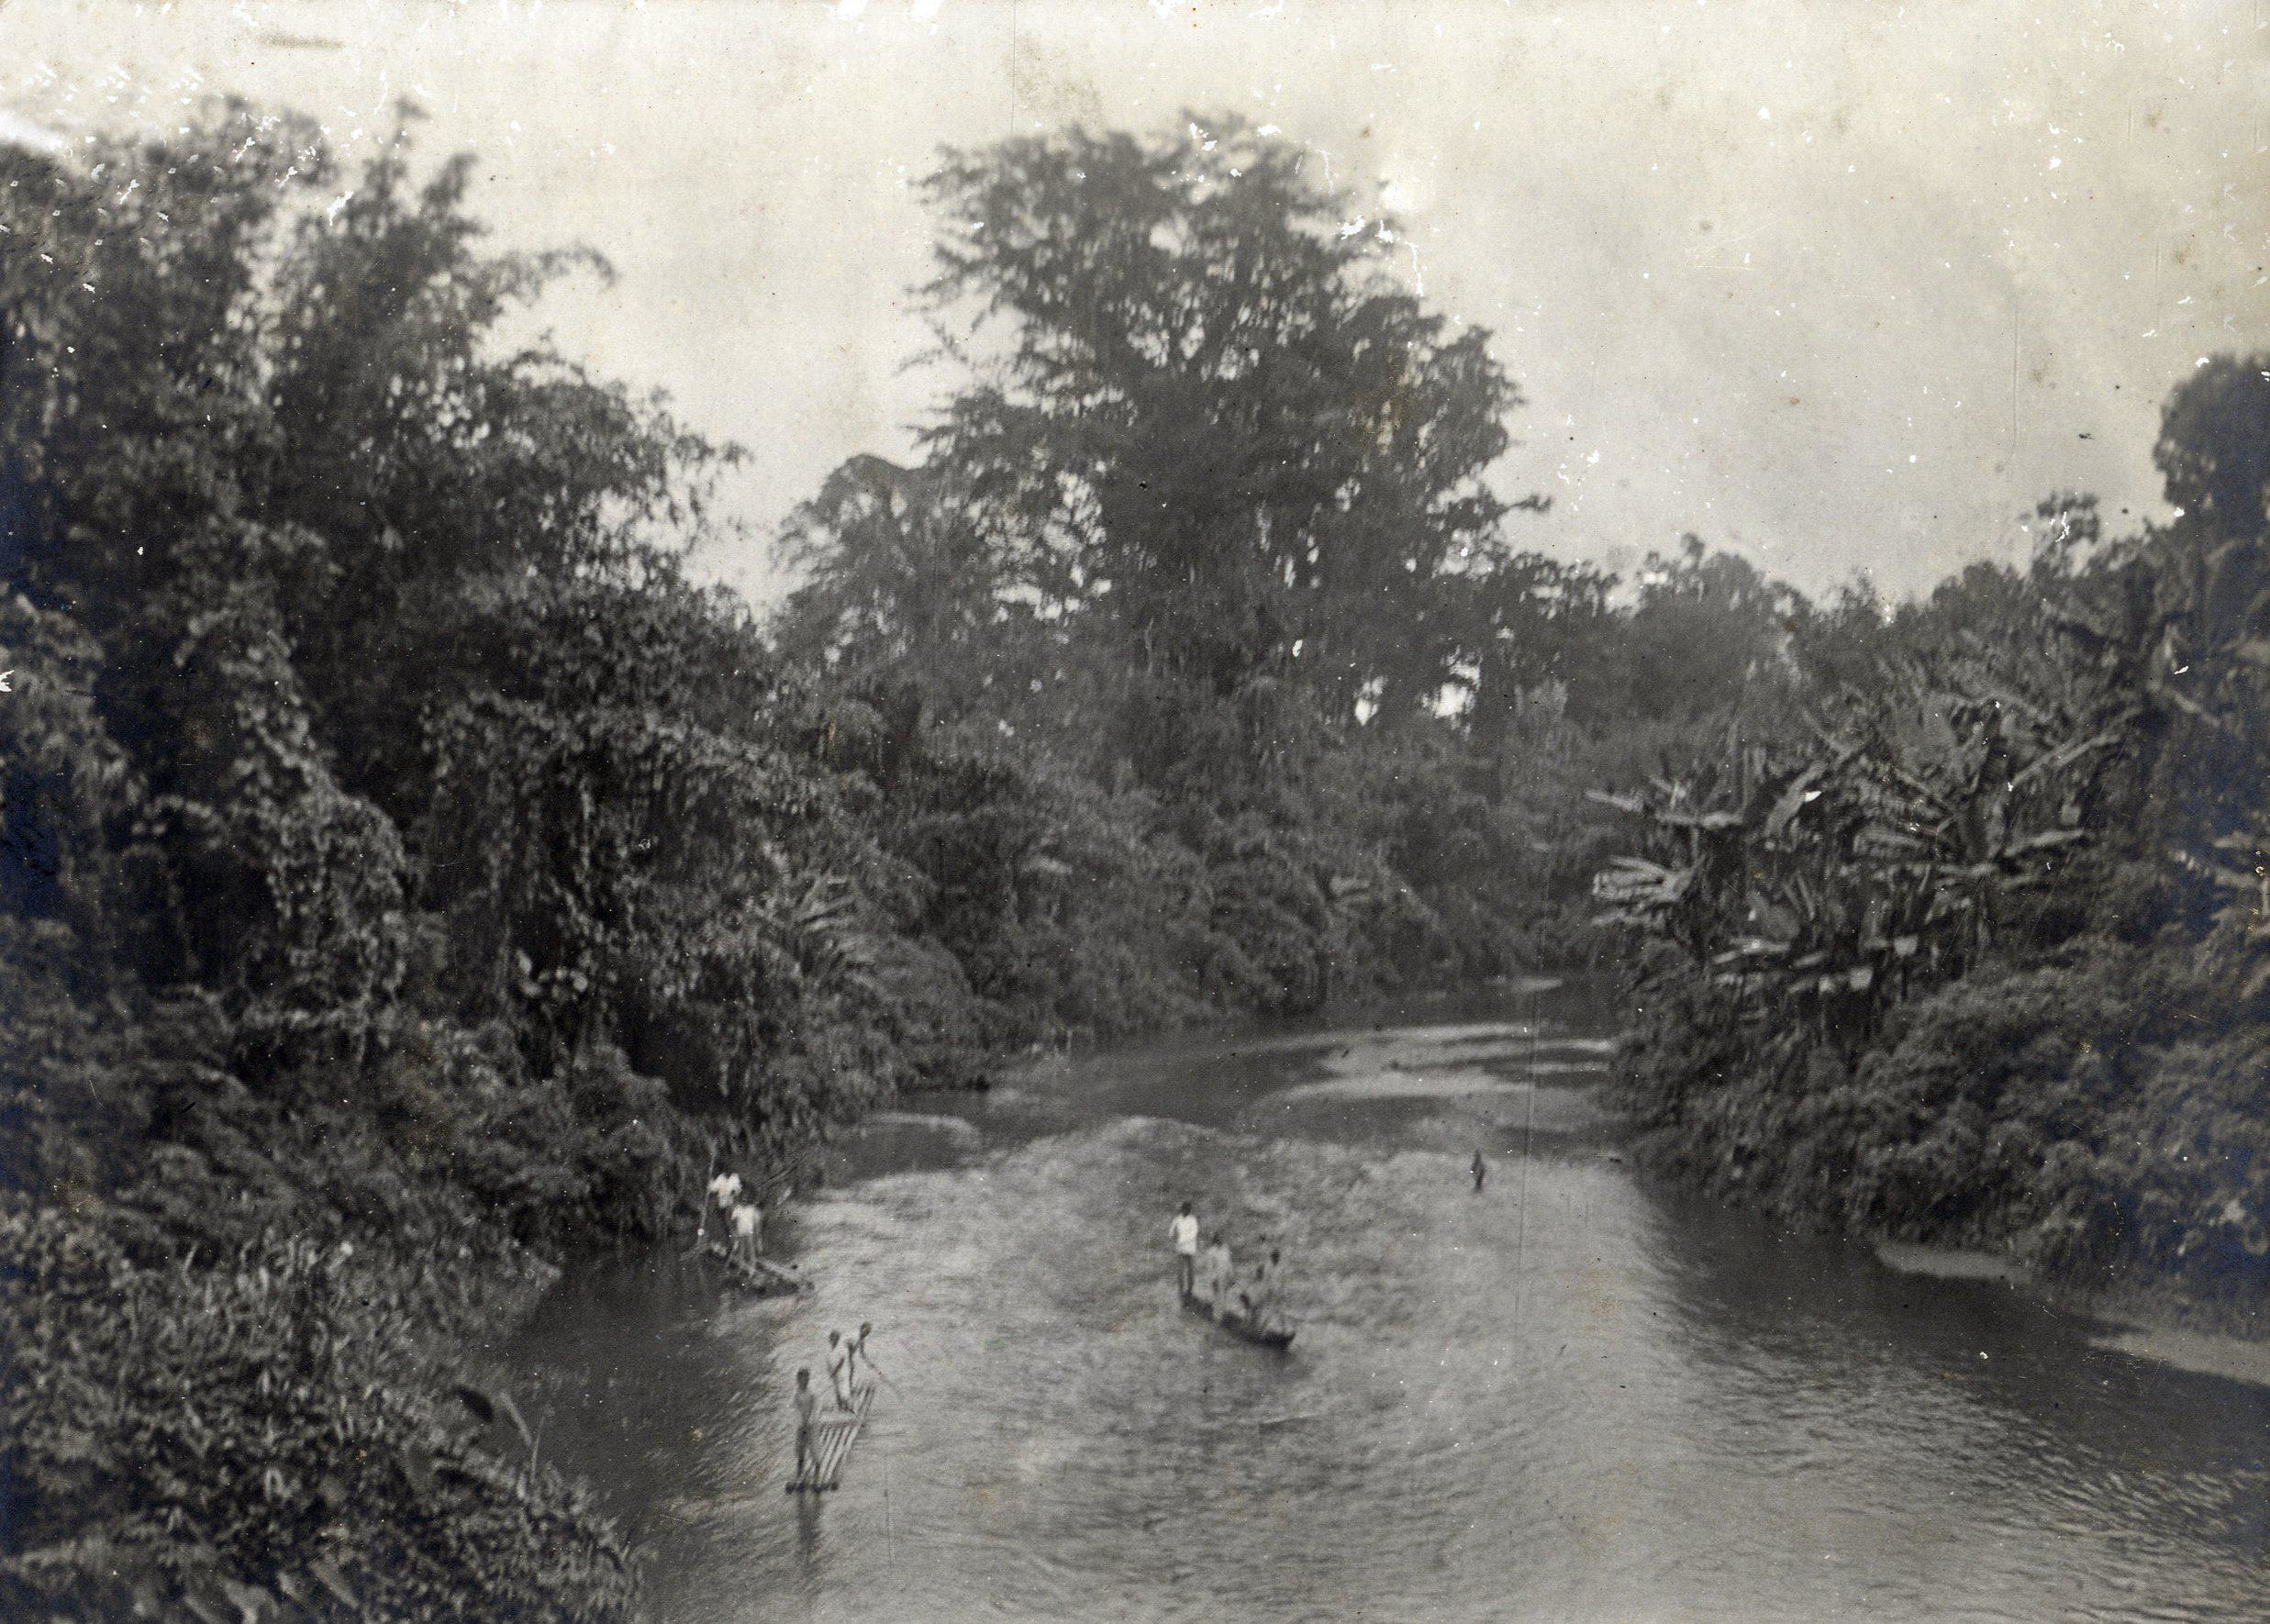
\includegraphics[width=1\linewidth]{figures/Kao_river.png}
    \caption{Photograph titled \textit{Kano op de Kaoe-rivier in Halmahera} (`Canoe on the Kao river on Halmahera') from the KITLV archive (dated ca. 1910). [Public domain]}
    \label{fig:Kao_river}
\end{figure}

Modole villages were centered around a community house that also served as village temple. Houses were made of bamboo and built on poles (compare \textref{chapter:text09}). A photograph of such a house (though belonging to a family from the neighboring ethnic group called ``Tugutil''\footnote{``Tugutil'' is commonly used for Tobelo-speaking groups living in the interior of Halmahera. According to \citet{duncan1997} the name is regarded as offensive by people it is applied to.}) from the KITLV archive in Leiden is displayed in Figure \ref{fig:Tugutil_house}.\footnote{Link to the photograph: \url{http://hdl.handle.net/1887.1/item:827860} (accessed 4 October 2025)} 
The people also spent an extensive amount of time in their gardens (compare \textref{chapter:text02}, \textref{chapter:text04}) that were cultivated through swidden agriculture (see \cite{leith1999}, \cite[214-215]{hueting1922}). 

\begin{figure}
    \centering
    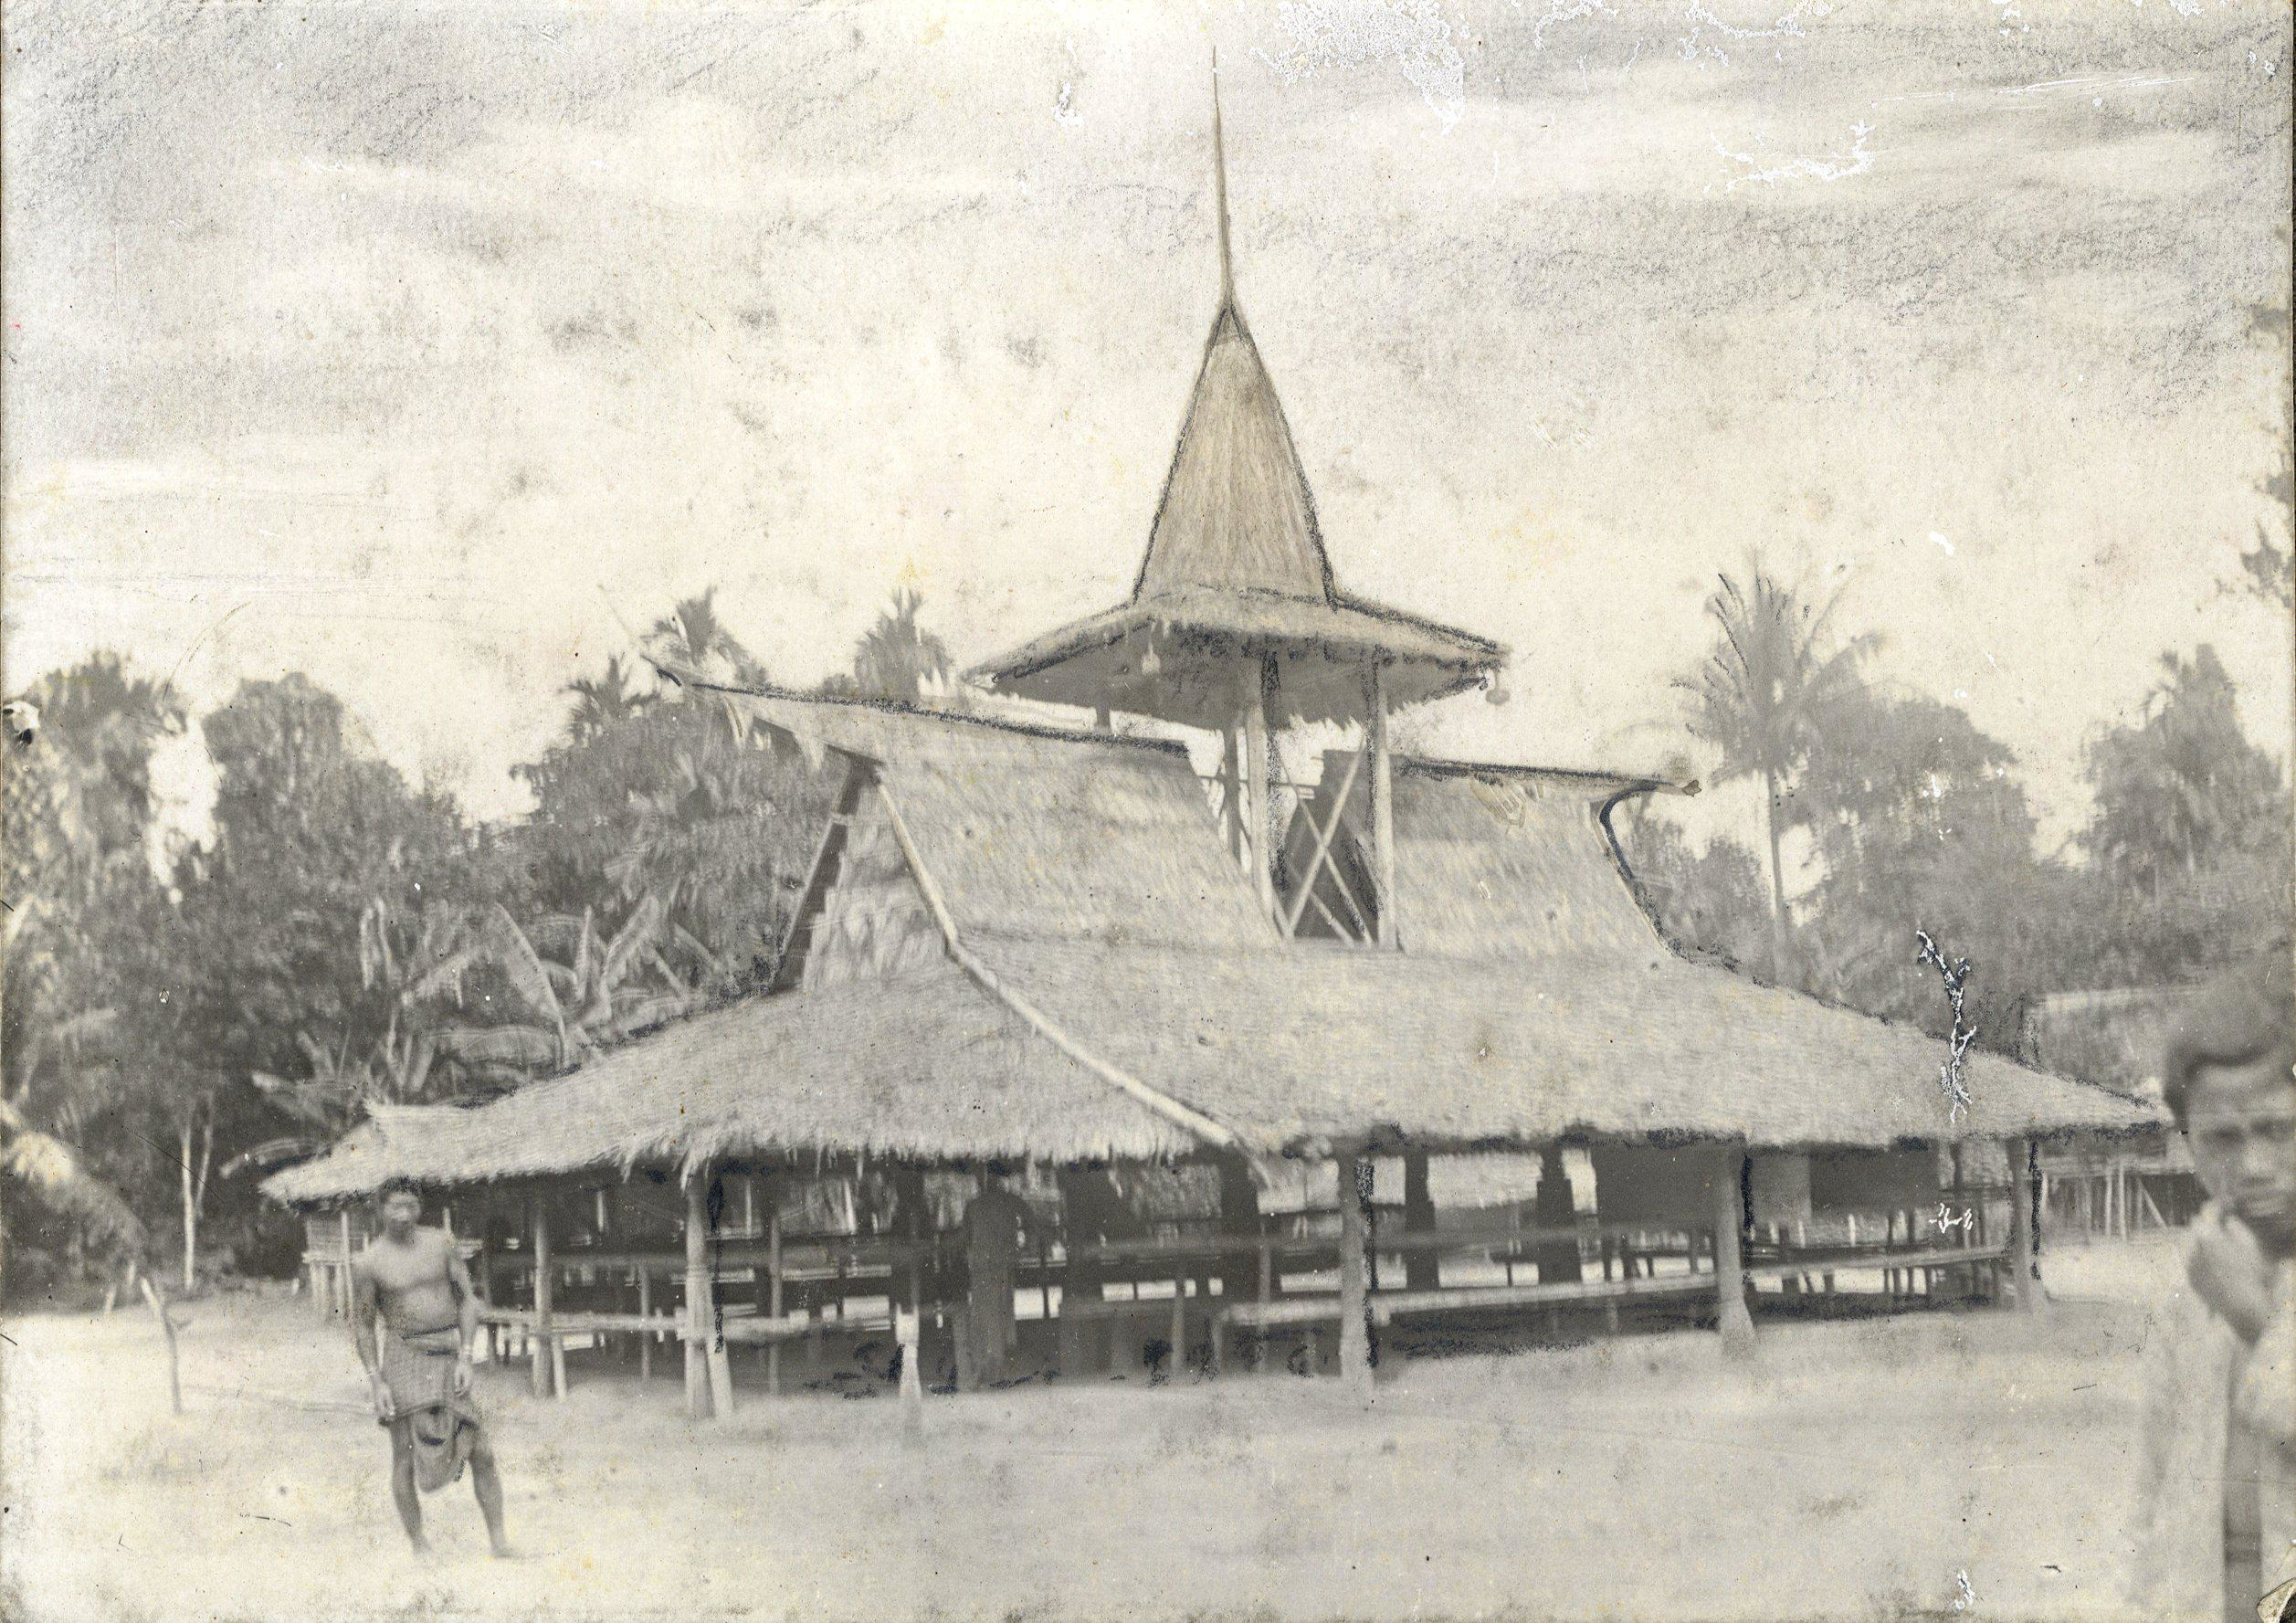
\includegraphics[width=1\linewidth]{figures/House.png}
    \caption{Photograph titled \textit{Gebouw te Toegoetils in Halmahera} (`Building of the Tugutils in Halmahera') from the KITLV archive (dated ca. 1910). [Public domain]}
    \label{fig:Tugutil_house}
\end{figure}

\section{The Modole language}
\label{sec:language}

\noindent Modole [mqo] (in some sources spelled Madole) is a Papuan language belonging to the North Halmahera language family. A map of the North Halmahera languages from 1908 can be found in Figure \ref{fig:NH_map}. Modole probably never had more than about 2,000 speakers -- the number of members of the group recorded throughout the early twentieth century until today.

Daily use of Modole is decreasing as speakers are shifting to North Moluccan Malay, the local variety of Malay and nowadays the major language of the North Moluccas  (see \cite{litamahuputty2012}). 
According to my Modole informant, Modole is still the main language in the villages of Kai, Pitago and Bailengi and children growing up there acquire Modole as L1. Modole speakers also have varying proficiency in Standard Indonesian and other local languages.

Modole is closely related to the other Core North Halmahera languages\footnote{This group includes all North Halmahera languages besides West Makian. I reconstruct their common ancestor as Proto-Core North Halmahera (\textsc{pcnh}).}, especially to those spoken on Halmahera proper (Mainland North Halmahera). Within the Core North Halmahera family, it subgroups with Tabaru and Pagu, which it closely resembles (see \citet{fortgens1928} for a description of Tabaru and \citet{peranginangin2018} for a description of Pagu). 
All Mainland North Halmahera languages are to a certain degree mutually intelligible and have been described as a continuum of dialects of the same language by \citet{voorhoeve1988}.
In 1910, G.J. Ellen reported that Tobelo was understood everywhere in the Kao ressort \citep[115]{ellen1910}. It is unclear whether this is due to mutual intelligibility of all languages in the area or because people were simply bilingual. 

According to \citet[189]{voorhoeve1988}, there is a northern and a southern dialect of Modole. The southern dialect has retained Proto-Core North Halmahera *s as /s/ while the Northern dialect has changed it to /h/.
In the 1980s, Northern Modole was spoken in the villages of Kai, Pitago, Bailengit, Soa-ma-etek, Parseba and Tuguis, while southern Modole was spoken in Soahukum, Tolabit-Torawat and Soasengaji (today called Sangaji Jaya).

Modole has borrowed a large number of lexical items from the local lingua franca Ternate and the wider lingua franca Indonesian. Other sources of loan words include Javanese (see Section \ref{subsec:folk_religion}) and European languages such as Portuguese and Dutch. Some loan words are indicated in the footnotes to the texts. 

Publications in and about Modole are scarce. The UZV missionary G.J. Ellen published a wordlist \citep{ellen1916b} with around 1,000 entries and the text collection edited in this book \citep{ellen1916}. In the late 19th century, Dutch colonial administrator K.F. Holle initiated the collection of wordlists for several Indonesian languages. The project was continued after his death and the wordlists are published in \citet{stokhof1980,stokhof1980a}. The Modole wordlist contains about 700 entries. The list is mentioned in the 1933 \textit{Jaarboek} of the \textit{Bataviaasch Genootschap van Kunsten en Wetenschappen} and it was likely collected between 1926 and 1932. The time and place of recording are unknown, as is the name of the recorder, but it is likely that Ellen was involved. The Holle wordlist deviates in some points from Ellen's wordlist.
In 1976, Yuiti Wada collected wordlists covering a total of 229 entries with two Modole speakers (published in \cite{wada1980}). In 1980, C.L. Voorhoeve recorded a wordlist and a short narrative in Modole. The recordings are now archived in PARADISEC.\footnote{See \url{https://catalog.paradisec.org.au/collections/CLV1/items/245} for the wordlist and \url{https://catalog.paradisec.org.au/collections/CLV1/items/260} for the continuation of the wordlist and the narrative (both accessed 4 October 2025).}
\citet{voorhoeve1988} includes some general remarks about the geographic and dialectal distribution of Modole. 
A Bible lesson was recorded in 2022 with a Modole speaker from Soamaetek for \citet{globalrecordings2023}.\footnote{I am grateful to Edward Kotynski for providing me with this information.} There is also a Modole version of the Jesus film \citep{jesusfilmprojectnd}. 
In 2024, the Indonesian government organization \textit{Badan Riset dan Inovasi Nasional} (BRIN) conducted linguistic research in the Modole village of Soamaetek, lead by Dyah Susilawati.\footnote{Personal communication with Dyah Susilawati, 12 January 2025}
As of September 2025, a Bible translation project is ongoing.
All these publications and projects are concerned with the northern dialect of Modole.

\begin{figure}
    \centering
    \includegraphics[width=.9\linewidth]{figures/Hueting1908.png}
    \caption{Approximate position of the North Halmahera languages in 1908, based on \citet{hueting1908}. [created by the author]}
    \label{fig:NH_map}
\end{figure}

\chapter{G.J. Ellen and the Halmahera mission of the Utrechtse Zendingsvereeniging}
\label{chap:Ellen}

Gerrit Jan Ellen (1876-1957)\footnote{see \url{https://webggc.oclc.org/cbs/DB=2.37/XMLPRS=Y/PPN?PPN=33831444X}, \url{https://hetutrechtsarchief.nl/collectie/AF6E16D8195046BB9CFADC700C5F24C9} (both accessed 4 October 2025)} was a missionary of the Utrechse Zendingsvereeniging (UZV; established 1859). This organization was part of the Protestant Dutch Reformed Church.
Information about Ellen's mission can be gathered from several publications: \textit{Handelingen der Utrechtsche Zendingsvereeniging}, \textit{Berichten van de Utrechtsche Zendingsvereeniging} as well as Ellen's (\citeyear{ellennda}) autobiographic report of his mission titled \textit{Uit mijn ervaring} (`From my experience'). For a history of the UZV mission in general see \citet{hueting1930}.
Ellen came to Halmahera in 1903 and worked there until he retired in 1938 \citep[188]{zendingsstudieraad1938}. 
For some years, he was accompanied by his wife N. Ellen-de Jong and (at least) two daughters born on Halmahera.
A picture of Ellen among his missionary colleagues is reproduced in Figure \ref{fig:conference}.\footnote{Link to the photograph: \url{http://hdl.handle.net/1887.1/item:827841} (accessed 4 October 2025)}

\begin{figure}
    \centering
    \includegraphics[width=1\linewidth]{figures/Zendelingenconferentie.jpg}
    \caption{Photograph titled \textit{Zendelingenconferentie te Tobelo in Halmahera} (`Missionary conference at Tobelo in Halmahera') from the KITLV archive (dated ca. 1910). The person identified as Ellen is circled. [Public domain]}
    \label{fig:conference}
\end{figure}

Within a few months of his arrival, he was allocated the Kao ressort. It covered the coast and interior north of Kao bay, that is the southern Tobelo settlements (Tobelo Boeng) and inland areas occupied by Pagu and Modole. In 1914, this ressort included 25 congregations with 2735 members \citep[136]{utrechtschezendingvereeniging1915}.

Ellen settled in the proximity of a coastal village called Pupupi and called the settlement Gamlaha (Ternate for `beautiful village') in 1907.\footnote{This is still the official name of the village as of 2025.}
The place is located in the Tobelo-Boeng speaking area. Ellen did not spend much time in the interior. Trips there were arduous and therefore seldom made (see \citet{ellennd}).

Ellen made first contact with the Modole in 1906 and some villages showed interest in becoming Christians \citep{ellen1906}.
In 1908, the mission had already advanced significantly among the Modole. There now was a guru called G. Tetalepta placed at Bailengit. His purview included people from the nearby villages Gogola ma lako (where all people had become Christians with the exception of four families) and Tomarate. Some of the inhabitants of Tomarate had moved to Bailengit and the rest was expected to follow them. This, Ellen explained, was necessary since a guru could only be placed in larger settlements \citep[158]{ellen1908}.
Both Gogola ma lako and Tomarate do not feature on modern maps, indicating that they were eventually abandoned.
The KITLV archive in Leiden hosts a photograph titled \textit{Leraar met zijn familie te Bailengit bij Kaoe in Halmahera} (`Teacher with his family at Bailengit near Kau in Halmahera'); see Figure \ref{fig:guru}.\footnote{Link to the photograph: \url{http://hdl.handle.net/1887.1/item:830771} (accessed 4 October 2025)} It is unknown if the photograph shows G. Tetalepta or a different guru.

\begin{figure}
    \centering
    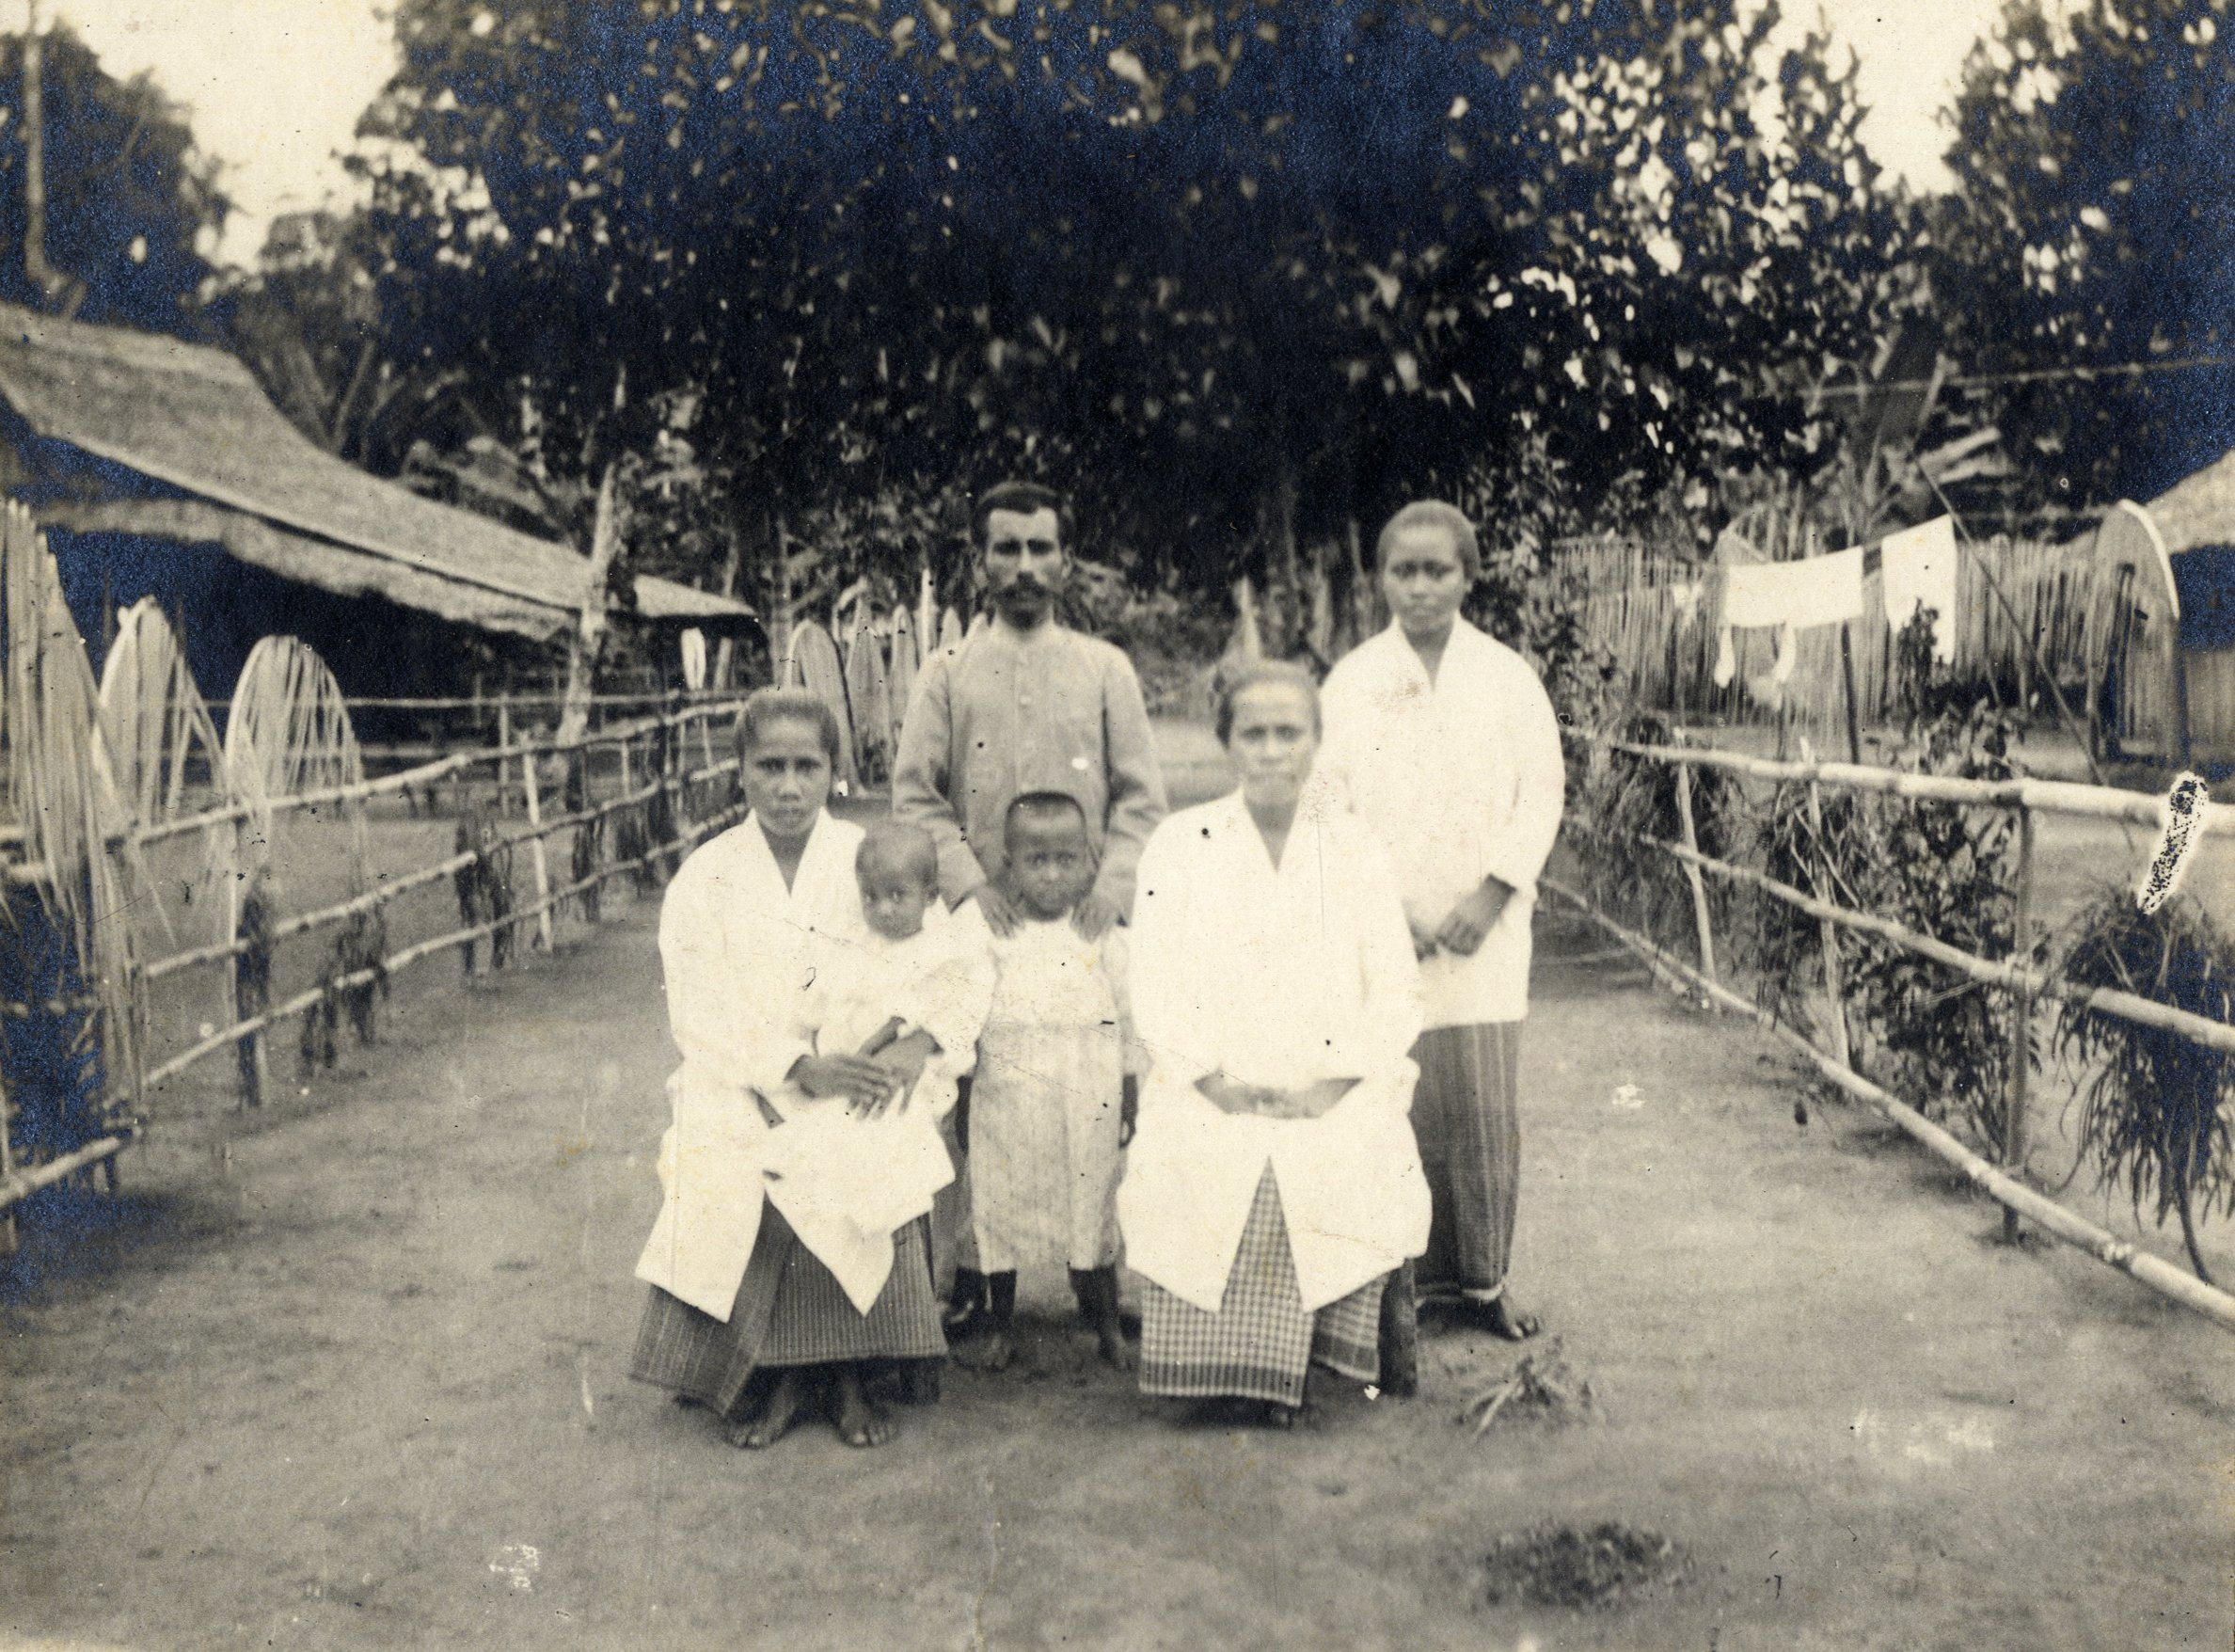
\includegraphics[width=1\linewidth]{figures/Guru_Bailengit.png}
    \caption{Photograph titled \textit{Leraar met zijn familie te Bailengit bij Kaoe in Halmahera} (`Teacher with his family at Bailengit near Kau in Halmahera') from the KITLV archive (dated ca. 1910). [Public domain]}
    \label{fig:guru}
\end{figure}

A guru by the name of P. Nanlohy was placed at Perseba. 
People in Toguis (Tuguis) were interested in Christianity while the inhabitants of Soamaetek still preferred to keep their native religion.
This had changed by 1918, when Ellen was able to report that almost everyone in Soamaetek was now baptized \citep{ellen1918}.

By 1908, Ellen had also visited the villages in the south Modole area: Soahukum, Tolabit and Soasengaji. People there were interested in Christianity but Ellen was unable to start work there since the villages had been partially abandoned due to recent unrest in the area \citep[159]{ellen1908}.
The people of Tolabit eventually converted in 1917 \citep[65]{leith1999}.
Today, most Modole are Christians.

As we can glean from his writings and published letters\footnote{These are letters he wrote to the council of the UZV published in the \textit{Berichten van de Utrechtsche Zendingsvereeniging}.}, Ellen's main goal in his work as a missionary was to enkindle a profound and personal Christian belief in the people of Halmahera. Further occupations of the UZV missionaries included the founding of schools (there were at least eight in Modole settlements by 1915) and the opening of income sources for the mission and the newly established congregations (for example coconut plantations). 
Ellen does not seem to have been particularly interested in linguistic and ethnological studies -- unlike some of his colleagues on Halmahera who published extensive dictionaries, grammatical descriptions and ethnological papers about the languages and people they encountered. 
Ellen preferred to discuss aspects of his mission in his writings. Information about the life of the people of Halmahera is only included whenever he laments the poor living standards. 
Information regarding Ellen's personal life is likewise absent. Even in his autobiographic work \textit{Uit mijn ervaring} \citep{ellennda} he does not discuss his life before he came to Halmahera or why he chose to become a missionary. I therefore know nothing about his educational background. Missionaries of the UZV went to a missionary seminar where, among other things, they studied Malay and sometimes also a local language relevant for their mission \citep{adriani1906}. Most likely, Ellen had no academic education in linguistics. 

\chapter{Provenance of the texts and this edition}
\label{chap:stories}

In this chapter, I attempt to shed some light on the provenance of the texts (\sectref{sec:provenance}). I also provide information on the structure and process of my edition of the texts (\sectref{sec:thisedition}).

\section{The provenance of the texts}
\label{sec:provenance}

As mentioned above, the provenance of the texts is unclear. 
Neither the story collection nor the accompanying wordlist \citep{ellen1916b} contains any information about who told the stories, and where and when they were recorded. To my knowledge, the Modole are now unfamiliar with the collection and preserve no memory of its recording.
Ellen first made contact with the Modole around 1906. He went on leave in July 1913 and stayed in the Netherlands until March 1915 (\cite{ellen1913, ellen1915}).
It is likely that he prepared and submitted the collection for publication during his stay in the Netherlands, which pinpoints their time of recording to between 1906 and 1913.

If Voorhoeve's (\citeyear{voorhoeve1988}) assertions are correct, the texts are recorded in the northern Modole dialect, since they reflect Proto-Core North Halmahera *s as /h/. This is even more likely since the northern Modole villages came under the influence of the mission at an earlier time than the southern villages (see Chapter \ref{chap:Ellen}). Potential places of collection are the villages of Perseba and Bailengit where gurus were placed at the collection time.

It is by no means certain that it was Ellen who wrote down the texts. Since Ellen did not spend much time in the Modole villages, they could well have been collected by one or more of the gurus who lived there permanently.\footnote{The archive of Ellen's UZV colleague J. Fortgens in Leiden hosts manuscripts in many different hands and some notebooks have the name of a guru on the cover.} 

I conducted no analysis of linguistic differences between the individual texts but it is notable that elements roughly meaning `then', used to structure the discourse, vary from text to text (see Table \ref{tab:discourse} for number of occurrences). 
The most frequent of these elements is \textit{geena('a) de} and it is the only one used in Texts \ref{chapter:text01} and \ref{chapter:text02}.  It is, however, absent from Texts \ref{chapter:text03} and (with one exception) Text \ref{chapter:text04}. These two texts use \textit{i'a} and \textit{ena} instead. The form \textit{geena'adau de} only occurs in Texts \ref{chapter:text05}, \ref{chapter:text06} and \ref{chapter:text07} and in Text \ref{chapter:text08} \textit{done} is used but does not occur in any other text.
This observation may be due to coincidence -- or it may point to different speakers, maybe even speakers from different villages. 

\begin{table}
    \caption{Discourse-structuring elements}
    \label{tab:discourse}
    \begin{tabularx}{.75\textwidth}{llllll}
        \lsptoprule
        &   \textit{geena'a de}&\textit{i'a}&  \textit{ena}&\textit{geena'adau de}&\textit{done}\\
        \midrule
        Text \ref{chapter:text01}&   7&--&  --&--  &--\\
        Text \ref{chapter:text02}&   8&--&  --&--  &--\\
        Text \ref{chapter:text03}&   --&1&  1&--  &--\\
        Text \ref{chapter:text04}&   1&8&  1&--  &--\\
        Text \ref{chapter:text05}&   2&--&  4&1  &--\\
        Text \ref{chapter:text06}&   4&3&  3&1&--\\
        Text \ref{chapter:text07}&   2&4&  --&4&--\\
        Text \ref{chapter:text08}&   3&1&  --&--  &2\\
        Text \ref{chapter:text09}&   1&--&  --&--  &--\\
        Text \ref{chapter:text10}&  --&--& --&--  &--\\ 
        \lspbottomrule
    \end{tabularx}
\end{table}

The background of the original editing and publication of the texts is as obscure as their collection. It is unknown whether Ellen translated the texts on his own or together with speakers of Modole. Ellen lived among Tobelo speakers and he was also acquainted with Pagu. With the help of the already published dictionaries and descriptions of other North Halmahera languages, he may have been able to produce reasonable translations on his own. There are several mistakes in the translation that point to this scenario. 

One mistake concerns the translation of a certain actor--undergoer combination. Modole shows a metathesis in the combination for a first person plural exclusive acting on a second person plural. Regularly, the form should be \textit{mi ni} and occurs as such in Pagu. Modole, on the other hand, has \textit{ni mi}. The Dutch translation mistook \textit{ni mi} for a second person plural acting on a first person plural exclusive in several cases.\footnote{Most of these cases are found in \textref{chapter:text04}. According to the Dutch translation, the ants ask the old people to search them for lice (\textsc{2pl>1pl.ex}). They then tell the old people to look up and throw lime into their eyes. This situation makes more sense if the ants search the old people who are seated with their back to the ants for lice (\textsc{1pl.ex>2pl}).} 
Ellen's translation should therefore always be checked with the original Modole text and the English translation provided by me.

\section{This edition}
\label{sec:thisedition}

For my analysis and translation of the texts, I used the FieldWorks Language Explorer (FLEx).\footnote{See \url{https://software.sil.org/fieldworks/} (accessed 4 October 2025)}
I copied the Modole text as well as the Dutch translation from an OCRed version of \citet{ellen1916} into FLEx and imported the available Modole wordlists (\cite{ellen1916b}, \cite{stokhof1980a}, \cite{wada1980}). I then compared the Dutch translation with the Modole text and the automatic matching of lexicon entries and word forms provided by FLEx. For unclear word forms or grammatical features, I checked dictionaries and descriptions of other North Halmahera languages. Some remaining questions were checked with a Modole speaker via an online messenger app. Unfortunately, it was not possible to check the complete translation with a Modole native speaker. 

Each of the texts is presented as follows in Chapters \ref{chapter:text01}--\ref{chapter:text10}. After a short introduction and summary of the text, I reproduce the Modole text in an adjusted spelling based on Indonesian orthography. This orthography is now used by Modole speakers, whereas not all of them are familiar with the Dutch-based orthography used by Ellen.\footnote{Notice that several grammatical items spelled separately by Ellen are nowadays conjoined with another word. It did not adopt this practise since there still is variation.} I have therefore given preference to the modern orthography here as well as in my morphemic analysis (see below) and the sketch grammar.
Deviations from the orthography used by Ellen are displayed in \tabref{tab:orthography}. 

\begin{table}
    \caption{Deviations between Ellen's and contemporary Modole orthography}
    \label{tab:orthography}
    \begin{tabularx}{.7\textwidth}{XXX}
        \lsptoprule
        \textsc{phoneme}&\textsc{ellen}&\textsc{contemporary}\\
        \midrule
        /j/& <dj> & <j>\\
        /c/&  <tj>& <c>\\
        /y/& <j> & <y>\\
        /ny/ & <nj> & <ny> \\
        \lspbottomrule
    \end{tabularx}
\end{table}

The letters <a> and <o> are often confused. This may be due to inconsistencies in transcription or typos introduced by the printers. I have not corrected any typos in order to preserve the original text but I have adjusted punctuation regarding direct speech. In the Modole text, colons and parentheses are often absent even where they occur in the Dutch translation. I inserted them so that now the Modole text and the Dutch as well as English translation correspond. I have not changed punctuation otherwise, even though it does not always feel adequate to the Modole language.\footnote{Commas and semicolons in the Modole text likely reflect Dutch conventions rather than breaks, for example.} 
Line breaks were introduced rather heuristically and are based both on Modole conjunctions such as \textit{de} `and', and punctuation.

Next is my English translation, which is based on the Modole text and differs in many points from Ellen's Dutch translation in the next section. See above for how I arrived at this translation.
The Dutch translation is faithful to the translation in \citet{ellen1916} with the exception of the addition of some missing colons and quotation marks. 

Next comes the interlinear glossed Modole text. The interlinear glossing is structured as follows:
The first line is the original Modole text and in most regards faithful to \citet{ellen1916}. Ellen's Dutch-based orthography is preserved here but missing colons and parentheses are added.
The second line presents my morphemic analysis (in modern orthography).
The third line contains the gloss of the morphemes found in the second line. In many cases, multiple glosses are possible. This is especially true for homographic morphemes like <ma> (`relational noun marker, `middle marker', `but', or `\textsc{3sgf>3nh}'), <o> (`noun marker', or incorrect spelling of the emphatic morpheme \textit{'o}) and <'a> (locative \textit{-o'a}, limitative \textit{-o'a}, or \textsc{itive} directional \textit{-i'a}). I was often left to guess and the glossing of these morphemes should hence always be taken with a grain of salt. Question marks indicate unclear glosses. Glosses are solely used as labels for often broader functions. For an analysis, the reader is pointed to the grammar sketch. 

The translation in the fourth line is more literal than the one presented above. I tried to imitate the original syntax as much as possible which in several cases leads to unidiomaticity in English. Most notably, I consistently translate the Modole directionals \textit{o'o} and \textit{iha} as `landward' and `seaward', respectively, in an attempt to reproduce this very prevalent feature of spatial orientation (see Section \ref{sec:directionals_locationals}). Punctuation follows the Modole original and hence is often inconsistent.
Uncertain translations are preceded by a question mark and alternative translations are discussed in the footnotes in the interlinear version of the texts.

\section{Overview of the texts}

\tabref{tab:texts} provides an overview of the texts included in this collection.

\begin{xltabular}{\textwidth}{lXr}
    \caption{The texts in this collection.} \label{tab:texts}\\

    \lsptoprule
        \textsc{text} & \textsc{title} & \textsc{words}\\
    \midrule
    \endfirsthead

    \multicolumn{3}{c}%
    {\tablename\ \thetable{} -- continued from previous page}\\
    \lsptoprule
        \textsc{text} & \textsc{title} & \textsc{words}\\
	\midrule
    \endhead

    \hline \multicolumn{3}{r}{{Continued on next page}}\\
    \endfoot

    
    \endlastfoot

    %\ref{chap02}&Clan history&&\textbf{2576}\\
		\ref{chapter:text01}&\textit{O lagudi ma howo’o wo djaga-djaga’a} - The guardian of the \textit{legundi} fruits&817\\
        \ref{chapter:text02}&\textit{O bibiti} - The \textit{bibiti} fish&699\\
        \ref{chapter:text03}&\textit{O Goda} - The \textit{goda} spirit&279\\
        \ref{chapter:text04}&\textit{O Gogunane} - The ants&658\\
        \ref{chapter:text05}&\textit{O lia’a de o dodoto} - The older and the younger brother&1161\\
        \ref{chapter:text06}&\textit{O uho} - The cuscus&1298\\
        \ref{chapter:text07}&\textit{O Biara} - The \textit{biara} plant&547\\
        \ref{chapter:text08}&\textit{Naga o njawa ja mididi jo puaha} - Two people who fasted&479\\
    %\ref{chap03}&Traditional stories&&\textbf{3531}\\
        \ref{chapter:text09}&\textit{O Lolabi mi tadi-tadi’a} - She is
stabbed by a kris&173\\
        \ref{chapter:text10}&\textit{Cumu cagulu} - Riddles&128\\
    \midrule    
        \textbf{total}&&\textbf{6239}\\
    \lspbottomrule
\end{xltabular}
